\chapter{Návrh riešenia}\label{chap:proposal}

Cieľom práce je detegovať reklamné plochy pri cestách z video záznamu a odhadnúť významnosť nájdených reklám. Významnosť reklám priamo súvisí s tým, na aký dlhý čas môže vodič stratiť pozornosť na ceste sledovaním danej reklamy.
\\

\begin{figure}[ht]
    \centering
    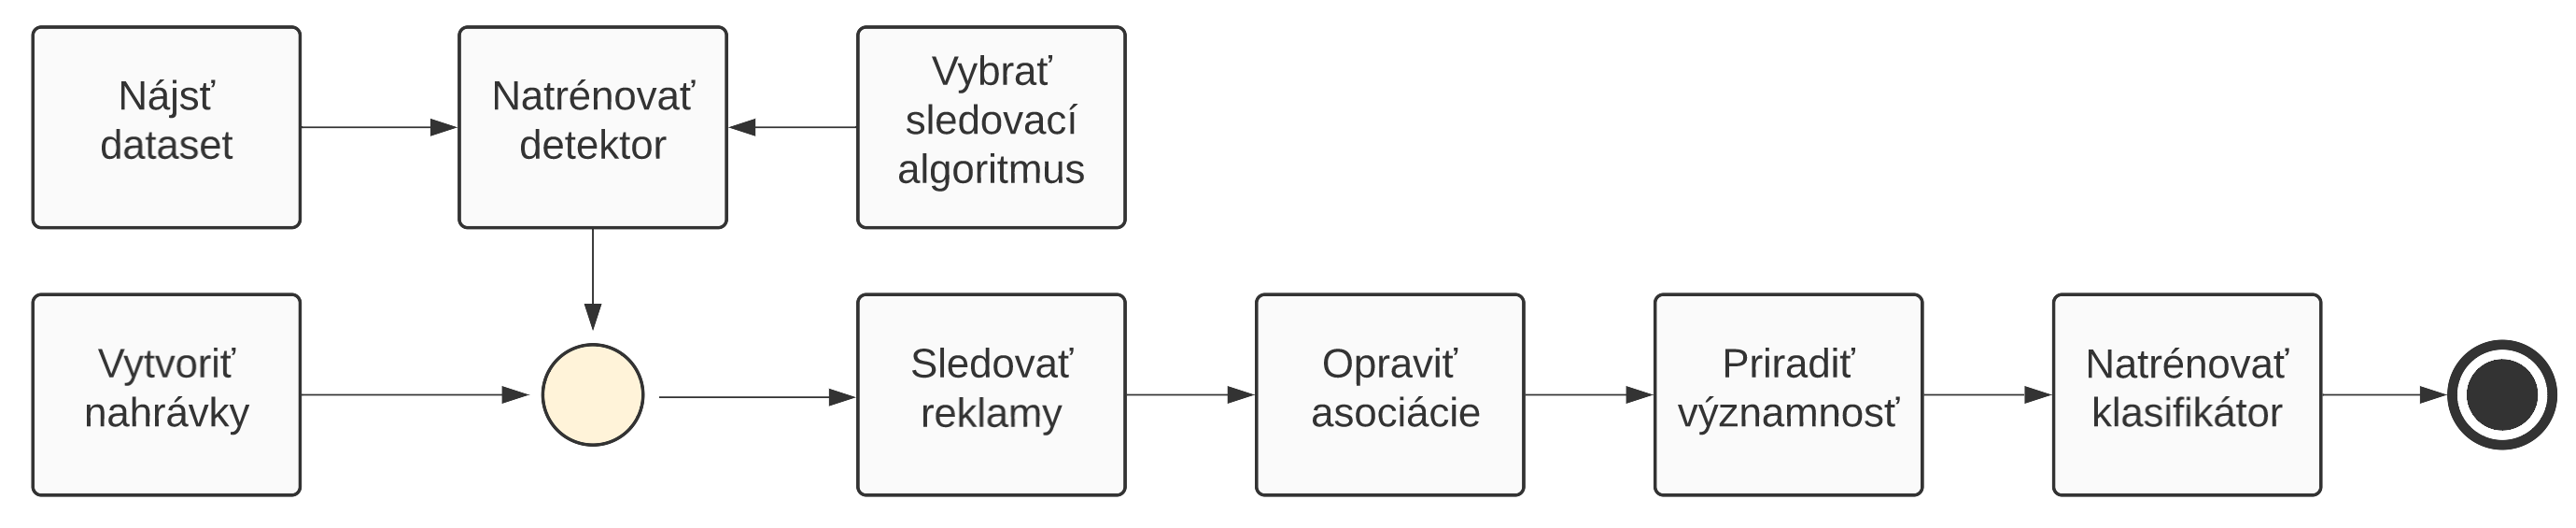
\includegraphics[width=1\textwidth]{images/02/plan2.png}
    \caption{Postup navrhnutého riešenia.}
    \label{img:road}
\end{figure}

\section{Príprava dát}

% Skôr než navrhneme spôsob, ktorým sa budú detegovať reklamy, potrebujeme vedieť s akými dátami budeme pracovať. 
Na fakulte školy máme k dispozícii eyetracker Tobii Glasses 3 \ref{img:tobii}, ktoré môžeme použiť na zber údajov. Eyetracker je zariadenie, ktoré dokáže snímať pohyb očí a súčasne nahrávať video. Výstupom je video záznam s informáciou, kam sa človek počas spusteného nahrávania pozeral. Dodatočnými informáciami sú otvorenosť očí a ďalšie údaje zo senzorov.

Kamera disponuje širokým záberom s rozlíšením 1920x1080. Na sledovanie pohybu šošoviek sú pripravené štyri kamery a ďalších šestnásť osvetľovačov. Všetko je integrované priamo v sklách okuliarov, pričom by nemali nijakým spôsobom brániť vo výhľade. Okrem toho sú sklá jemne zatienené, pretože sú veľmi citlivé na priame osvetlenie.

% TODO mať správne zapísané zdroje

\begin{figure}[ht]
    \centering
    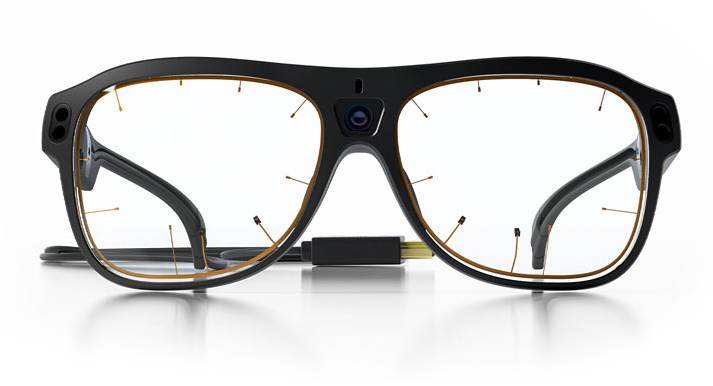
\includegraphics[width=0.6\textwidth]{images/02/glasses.jpg}
    \caption{Eyetracker, model Tobii Glasses 3 \cite{tobii}.}
    \label{img:tobii}
\end{figure}

% Pre náš výskum by sa dal základný scenár pre jeden záznam opísať tak, že si vodič nasadí eyetracker a následne šoféruje vozidlo po určitej trase. 
Pre účely práce potrebujeme vytvoriť viacero záznamov jednej trasy, ktorou pôjdu všetci vodiči. Navrhujeme preto základné podmienky pre experimentálne meranie, od ktorého očakávame dostatočnú kvalitu a kvantitu dát pre ďalší proces. Aby bolo meranie čo najviac konzistentné, je dôležité zabezpečiť rovnaké podmienky pre každého účastníka merania. 

Na základe prečítaných prác, ktoré robili podobný zber dát s vyhodnotením vieme povedať, že pohlavie neovplyvňuje meranie a preto, nezáleží na pomere pohlavia medzi účastníkmi. Naopak to čo meranie ovplyvňuje je vek účastníka a jeho skúsenosť so šoférovaním. Dôležitá podmienka je aj to, aby bola jazda v približne rovnakom počasí a s približne rovnakou hustotou premávky. 

% Na dosiahnutie nášho cieľa je vhodné, aby sa zvolila jedna trasa, ktorou pôjdu všetci vodiči. Ideálne taká, aby mala čo najviac reklám viacerých typov. 
Sledovaním reklám v našom okolí, sme nakoniec zvolili okružnú jazdu, ktorá je zobrazená na obrázku \ref{img:road}. Odhadovali sme, že na zvolenej trase, ktorá trvá približne 24 minút, sa môže vyskytovať približne 150 reklamných plôch. Trasa bola zvolená kvôli počtu reklám, ich rôznorodosti a jej blízkosti od fakulty.
\\
\begin{figure}[ht]
    \centering
    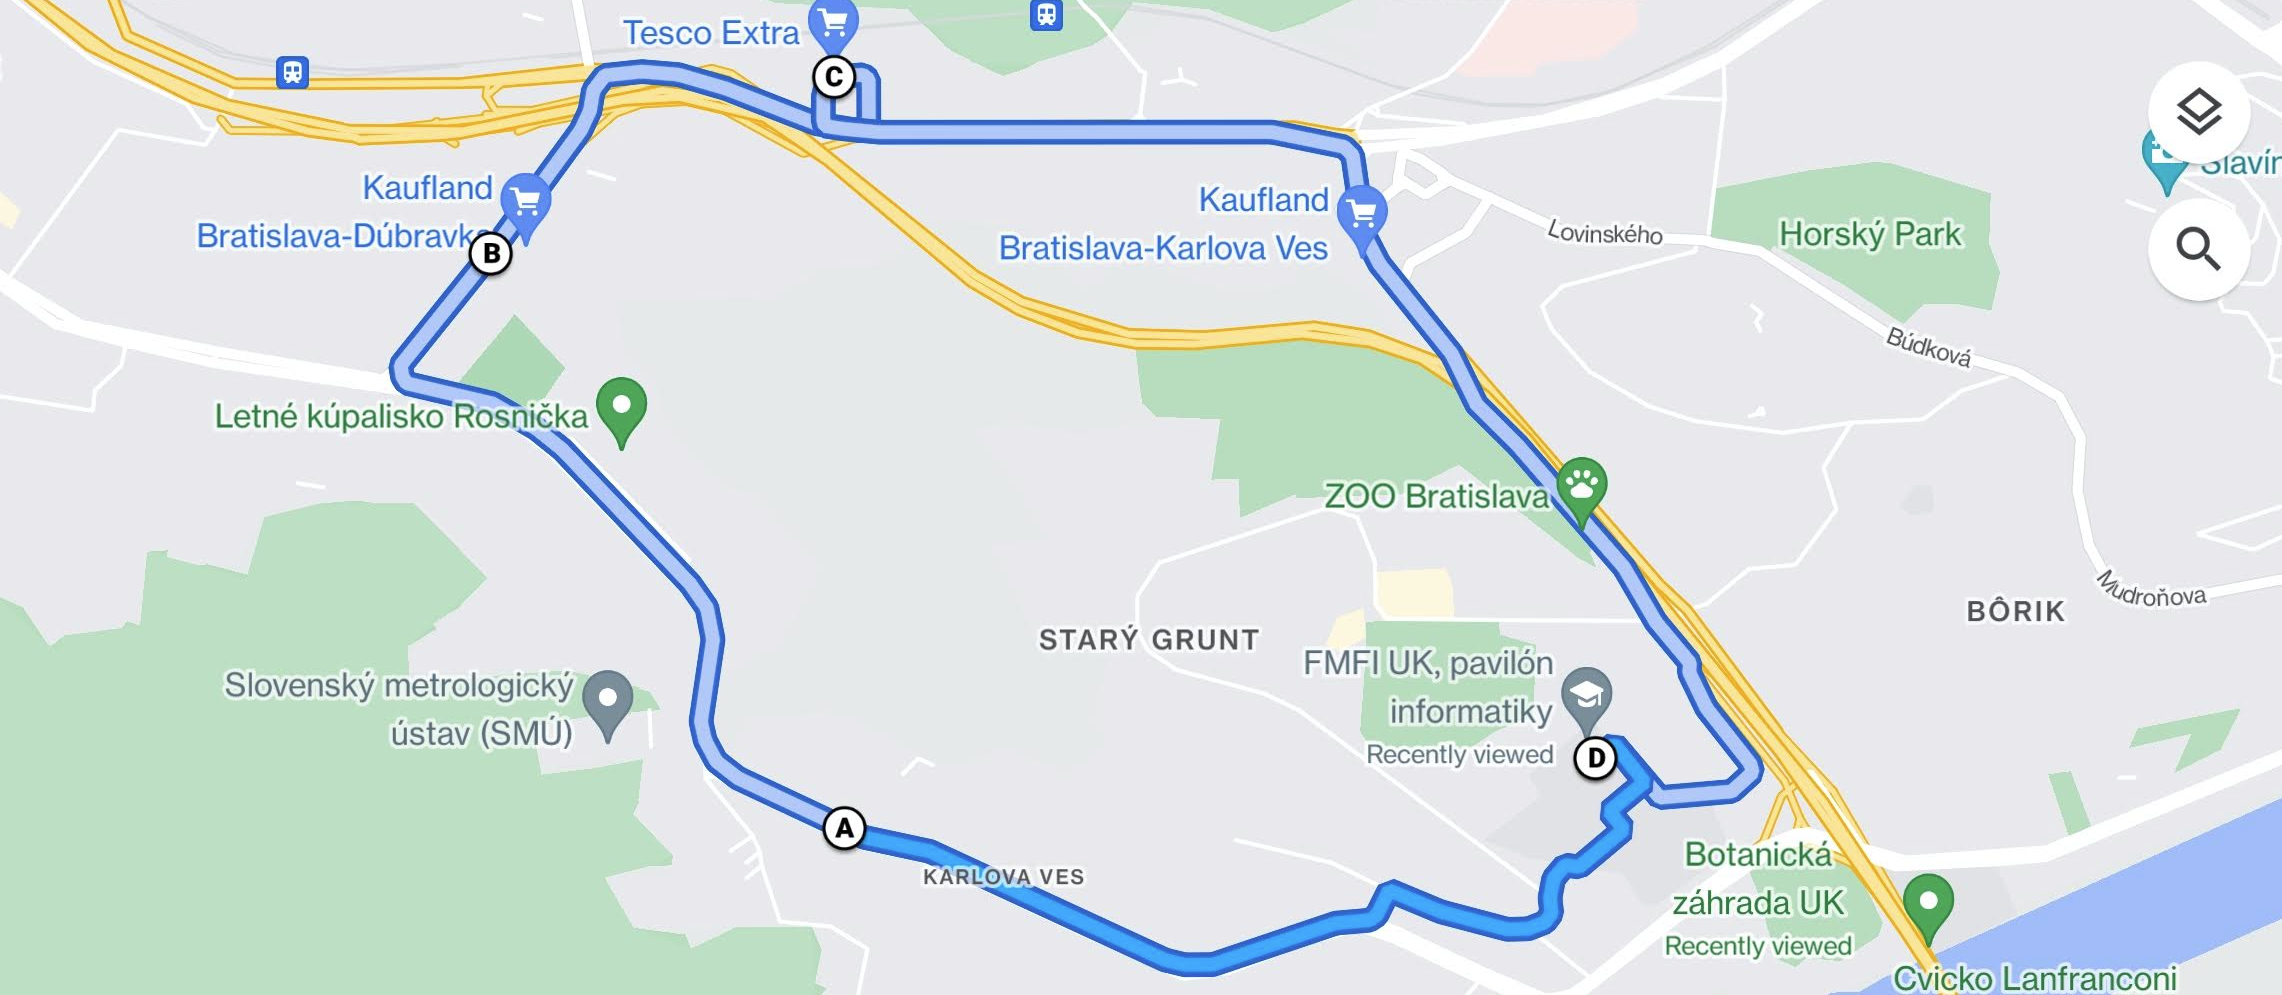
\includegraphics[width=1\textwidth]{images/02/map.png}
    \caption{Fixná trasa zvolená pre experimentálne meranie.}
    \label{img:road}
\end{figure}

\section{Detekcia reklám}

Na detekciu reklám využijeme konvolučnú neurónovú sieť. Zvolili sme YOLOv8 \cite{yolov8}, nakoľko bola predstavená na začiatku tohto roka so sľubným vylepšením oproti predchádzajúcim YOLO verziám. Na detekciu objektov, bude potrebné nájsť vhodný dataset, ktorý poslúži na trénovanie modelu.

% Na internete sme našli databázu bilbordov, ktorá mala takmer 4000 obrázkov. Bohužiaľ nevyhovovala našim potrebám, pretože obrázky boli vytvárané ako fotografie, kde reklama zaberala väčšinu plochy. 
Na trénovanie použijeme dataset Mapillary Vistas, ktorý bol uvedený v podobných prácach. Obsahuje anotácie pre 25000 obrázkov rozdelených do desiatok kategórií, medzi ktorými je trieda bilbord a banner. Obrázky sú zachytené zo strechy auta, v hustejšej premávke vo vnútri mesta, kde sa nachádza veľa budov, chodníkov a viacero dopravných označení. Nevýhodou môže byť vysoké rozlíšenie, na ktorom sú označené aj veľmi malé objekty.

% Jediný verejne dostupný dataset z podobných prác je Mapillary Vistas a vzhľadom na jeho veľkosť by to mohla byť dobrá voľba. Obsahuje 25000 obrázkov anotovaných do desiatok kategórií, medzi ktorými je aj bilbord a banner. Obrázky sú fotené v hustejšej premávke vo vnútri mesta, kde sa nachádza veľa budov, chodníkov a viacero dopravných označení. Nevýhodou môže byť vysoké rozlíšenie, na ktorom sú označené aj veľmi malé objekty.

\begin{figure}[ht]
    \centering
    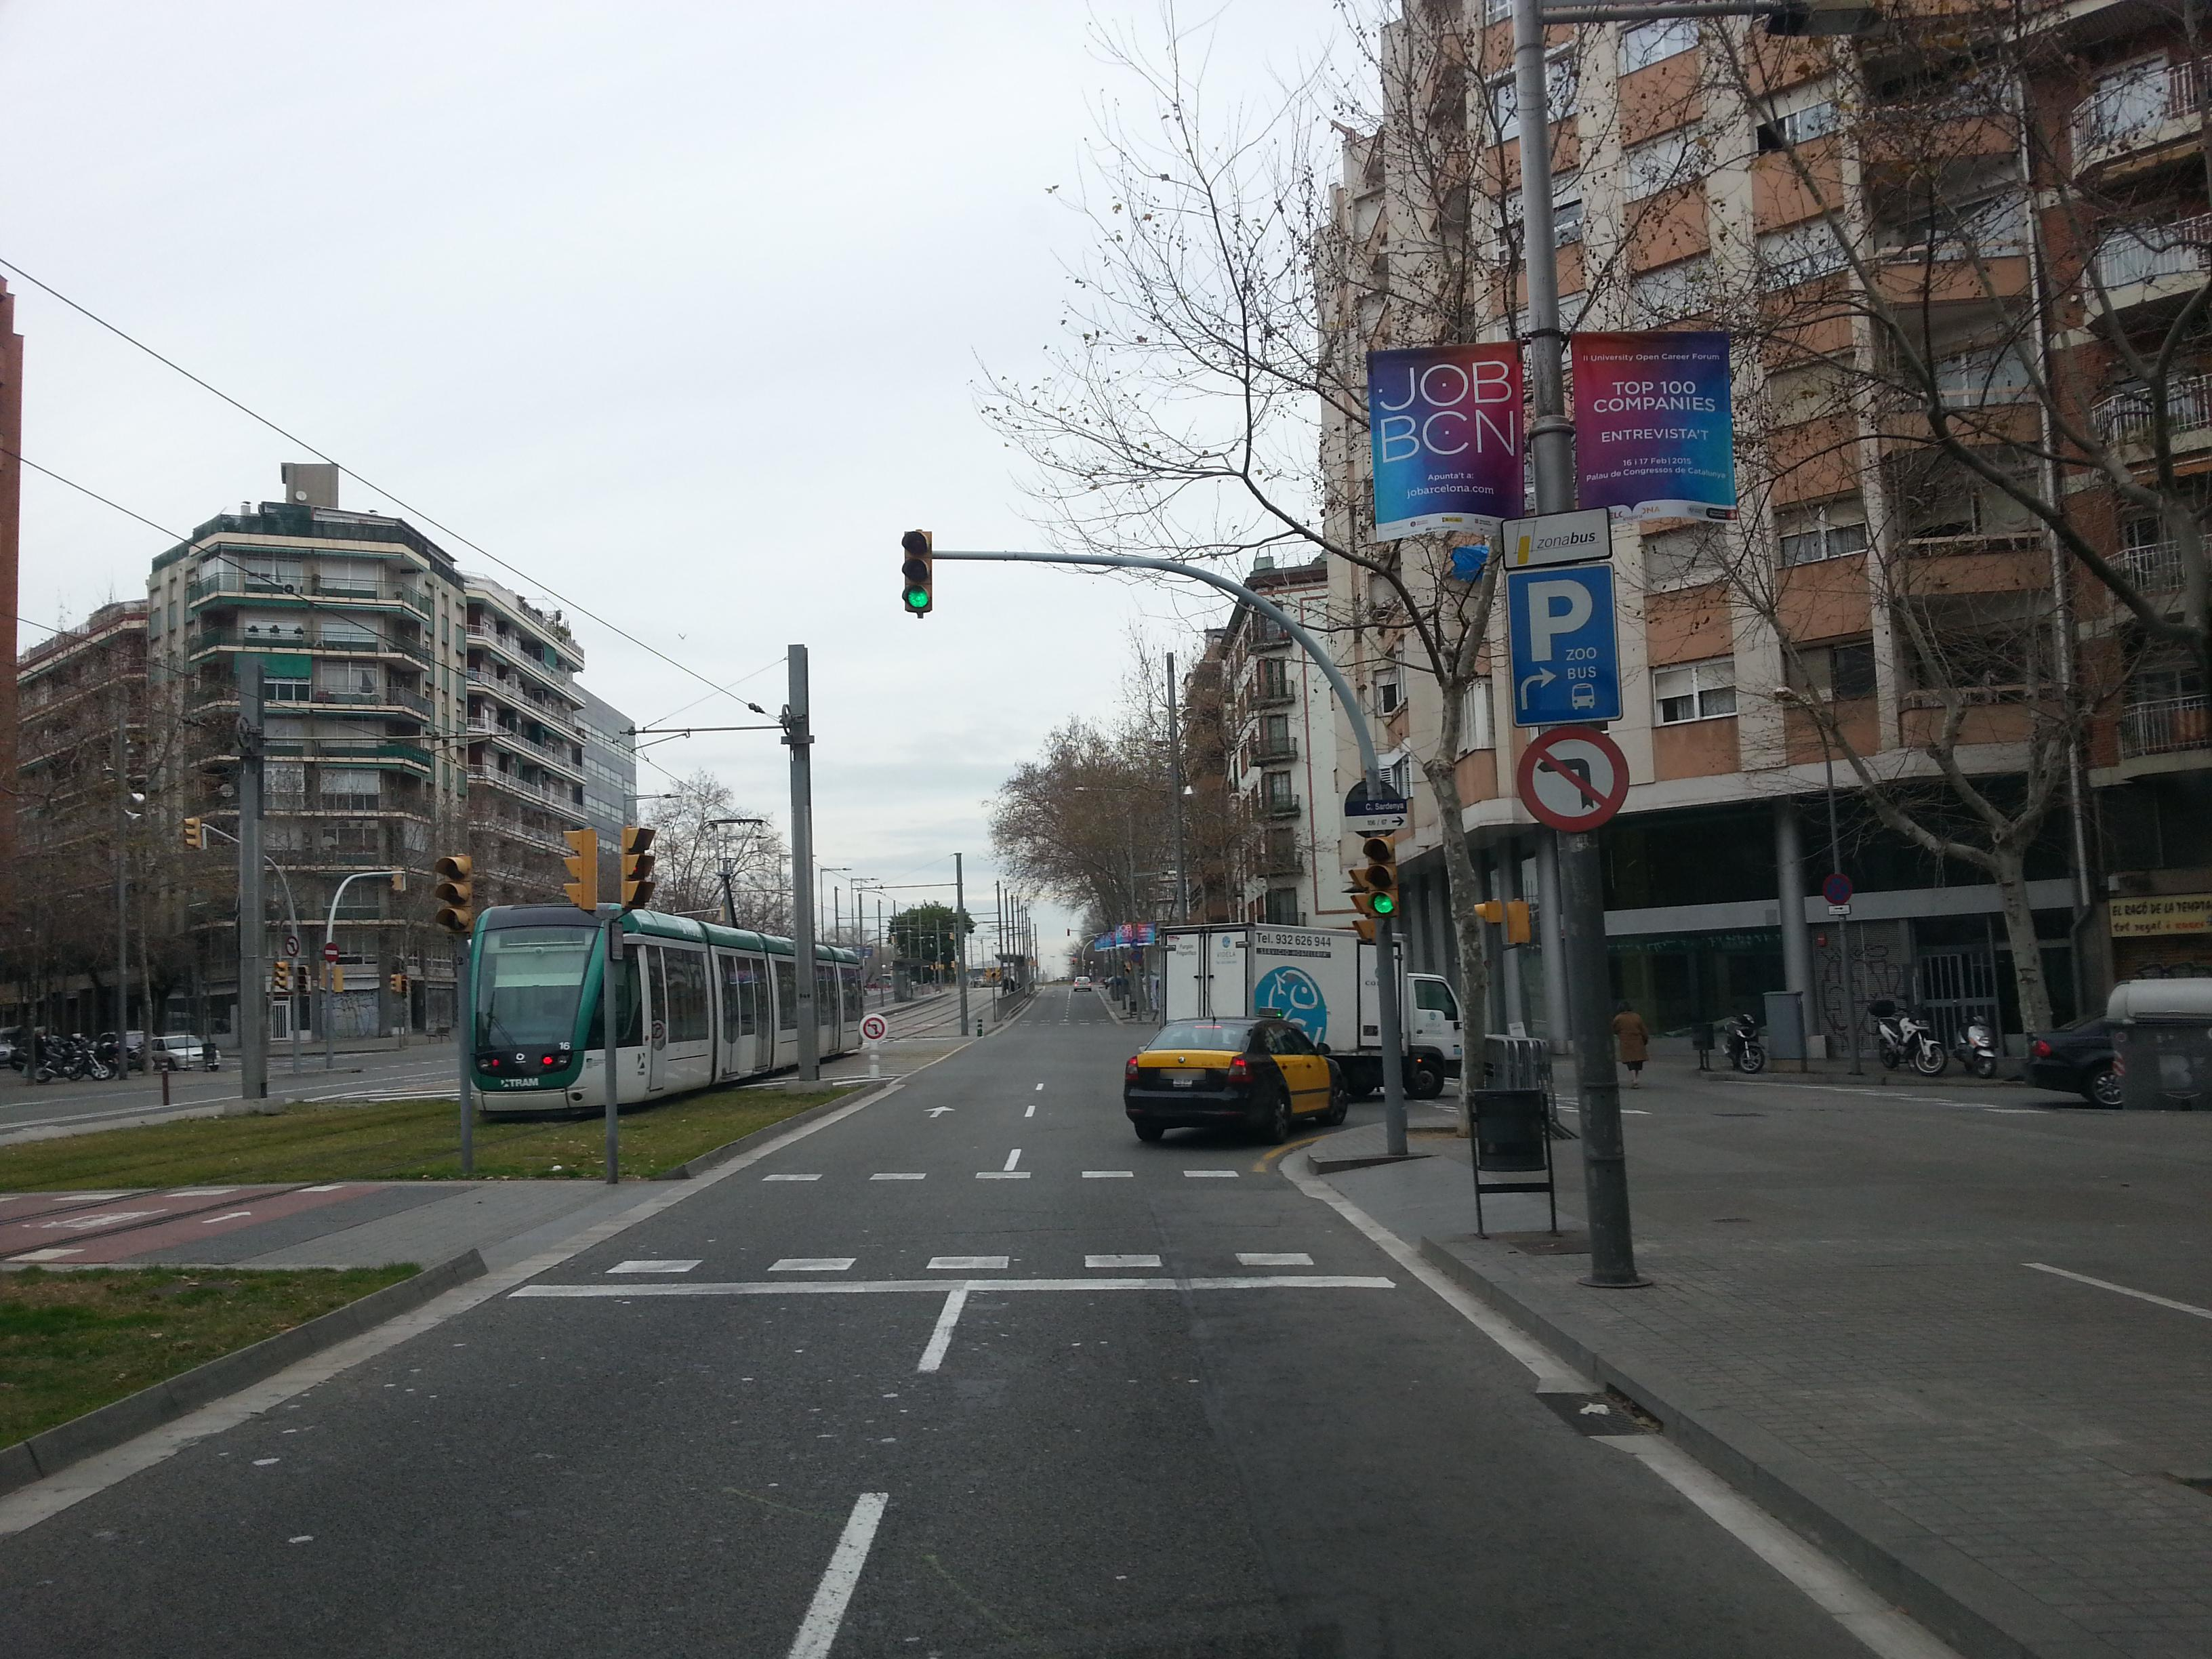
\includegraphics[width=1\textwidth]{images/02/mapillar.jpg}
    \caption{Ukážkový obrázok z datasetu Mapillary Vistas.}
    \label{img:dataset}
\end{figure}

\subsection{Sledovanie reklám}

Zatiaľ rozprávame o obrázkoch, ale nás v konečnom prípade zaujímajú video vstupy, preto potrebujeme zabezpečiť sledovanie objektov. 

Objekt nájdený vo videu sa dá sledovať pomocou sledovacích algoritmov založených na pohybe a asociácii. Tu môžeme vyskúšať viacero riešení a vyhodnotiť úspešnosť pomocou špecializovaných metrík. Sledovanie objektu sa líši voči detekcii tým, že pre nájdený objekt priradí identifikátor na základe asociácie s dostatočne podobným objektom. Ak sa zdá, že podobný objekt už bol na predošlých snímkach, tak mu priradí rovnaký identifikátor a ak nie, tak vytvorí nový. 

Medzi popredné modely na sledovanie objektov patrí Deep SORT \cite{deepsort}, ByteTrack \cite{bytetrack}, OC-SORT \cite{ocsort}, StrongSORT \cite{strongsort} a mnohé iné. Práve tieto uvedené modely vyskúšame a porovnané medzi sebou. Všetko sú to variácie modelu Simple Online and Realtime Tracking (SORT), ktorý na sledovanie používa Kalmanov filter a Hungarian algoritmus \cite{sort}.

% Samotný detektor objektov nedokáže sledovať reklamy. Samozrejme, že by mohol detegovať reklamy snímok po snímku, ale nedokázal by asociovať nájdený objekt priradením k jeho výskytu v predošlej snímke. 

% DeepSORT je rozšírením pre SORT, ktorý integruje informácie o vzhľade získané z predtrénovaného modelu. Výsledkom je lepšie priradenie správnej identity čo zároveň redukuje počet vytvorených identít \cite{deepsort}. ByteTrack sa zameriava na asociáciu údajov a navrhuje novú metódu Byte, ktorá sleduje priradenie s porovnávaním každého objektu, ktorý bol doposiaľ zaznamenaný \cite{bytetrack}. OC-SORT je metóda, ktorá používa pozorovanie objektov na výpočet virtuálnej trajektórie počas prekrytia objektu, aby sa zmiernilo hromadenie chýb Kalmanovho filtra, ktoré vzniká počas oklúzie \cite{ocsort}. StrongSORT je varianta, ktorá pridáva pohybový model založený na optickom toku na zlepšenie výkonu sledovania pričom sa snaží kombinovať výhody z metódy Deep SORT a ByteTrack \cite{strongsort}. Každý model má sadu parametrov, ktoré sme jemne upravovali a sledovali zmenu vo výsledkoch. 
% sorts: https://www.tasq.ai/blog/object-tracking/ 

\section{Významnosť reklám}

Pokiaľ detekcia, respektíve sledovanie dosiahne dostatočne dobrú úroveň, budeme vedieť nájsť zo záznamov také snímky, na ktorých sa nachádza reklama a spolu s nameranými pohľadmi vodiča pomenovať významnosť jednotlivých reklám. Pre každú nájdenú reklamu pomenujeme jej významnosť, čím vytvoríme malú databázu reklám. 

Urobíme to tak, že pre každú snímku, na ktorej bola nájdená reklama porovnáme prienik so získanou súradnicou miesta, kam sa vodič pozeral v danom okamihu pozeral. Pre každú reklamu tak získame informáciu o počte snímok, na ktorých bol prienik s pohľadom vodiča. Počet snímok vynásobíme dĺžkou trvania jednej snímky, čím získame časový údaj fixácie. Podľa dĺžky fixácie vyhodnotíme významnosť reklamy pre každého vodiča samostatne a následne vypočítame priemer. Významosť reklamy budeme rozdeľovať do jedenej zo štyroch kategórií: 

\begin{itemize}
  \item slabá: 0ms
  \item nízka: 1 - 99ms
  \item stredná: 100 - 299ms
  \item vysoká: 300ms a viac 
\end{itemize}

% používať číslo slovom alebo číslicou? napríklad.. to ako dlho vodič udrží pohľad na reklame časovo delia na 4\štyri kategórie

\subsection{Klasifikácia reklám}

Významnosť reklamy sa nakoniec budeme snažiť odhadnúť bez informácie o zaznamenanom pohľade vodiča. Na klasifikáciu použijeme klasické metódy zo strojového učenia, Random forest classifier (RFC), Support vector machine (SV) a K-nearest neighbours (KNN). 

Zo snímok na ktorých sa bude nachádzať reklama vypočítame niekoľko vlastností, samostatne pre každú reklamu. Zo sekvencie snímok by sa dali vypočítať napríklad tieto vlastnosť:

\begin{itemize}
  \item strana, na ktorej bola reklama (ľavo, stred, pravo),
  \item počet snímok, na ktorých bola reklama viditeľná
  \item priemerná vzdialenosť reklamy od stredu obrazu
  \item priemerná veľkosť reklamy v sekvencii
  \item priemerná hodnota z mapy významností pre reklamu v sekvencii
  \item pomer hodnoty významnosti reklamy s hodnotou v celej snímke
\end{itemize}

V záverečnom vyhodnotení sa bude dať zmerať úspešnosť sledovania reklám, vypočítaná významnosť reklám a napokon klasifikácia reklám.

% V konečnom dôsledku sa bude dať porovnať priradenie a odhad klasifikácie, čím určíme posledné sledované výsledky.

% Vykonať zber dát -> natrénovať detektor reklám -> sledovať reklamy z videa -> nájsť prienik reklám a pohľadov -> priradiť reklamám kategóriu významosti -> vytvoriť klasifikátor významnosti